\begin{flushleft}
Abbiamo scritto delle funzioni MalLab che ci permettono di effettuare il raffronto tra i vari metodi (in ordine: metodo di Newton, metodo di Newton modificato, metodo di accelerazione di Aitken), è possibile vederle a pag. \pageref{functcap2}. Scritte le Function, le abbiamo usate nel seguente script: 
\lstinputlisting[language=Matlab]{cap_2/es4/es4.m}
Questo codice esegue i metodi di Newton, Newton modificato e Aitken per le funzioni date. Rispetto alla funzione $f_1(x)=(x-\pi)^{10}$ rappresentiamo l'output del codice precedente in forma tabellare: 
\begin{center}
\begin{tabular}{|c|c|c|c|}
\hline
tolx & Newton & Newton modificato & Aitken \\
\hline
$10^{0}$ & 4.814159265358979 & 4.814159265358979 & 2.666666666666667 \\
$10^{-1}$ & 4.030463126315021 & 4.030463126315021 & 3.141592653589783 \\
$10^{-2}$ & 3.229126031324792 & 3.229126031324792 & 3.141592653589783 \\
$10^{-3}$ & 3.150212685926121 &  3.150212685926121 &  3.141592653589783 \\ 
$10^{-4}$ & 3.150212685926121 & 3.150212685926121 & 3.141592653589783 \\
$10^{-5}$ & 3.150212685926121 & 3.150212685926121 & 3.141592653589783 \\
\hline
\end{tabular}
\end{center}
Rispetto alla funzione $f_2(x) = (x-\pi)^{10} \cdot e^{2\cdot x}$ si hanno invece i valori:
\begin{center}
\begin{tabular}{|c|c|c|c|}
\hline
tolx & Newton & Newton modificato & Aitken \\
\hline
$10^{0}$ & 4.864516114854061 & 4.864516114854061 & 3.068982105941251 \\
$10^{-1}$ & 4.200823975656096 & 4.200823975656096 & 3.140645194956157 \\
$10^{-2}$ & 3.226469748549500 & 3.226469748549500 & 3.141592492095279 \\
$10^{-3}$ & 3.154537411727535 & 3.154537411727535 &  3.141592492095279 \\ 
$10^{-4}$ & 3.154537411727535 & 3.154537411727535 & 3.141592516390607 \\
$10^{-5}$ & 3.154537411727535 & 3.154537411727535 & 3.141592516390607 \\
\hline
\end{tabular}
\end{center}
Abbiamo poi riportato il plot matlab relativo ai precedenti valori:
\begin{figure}[H]
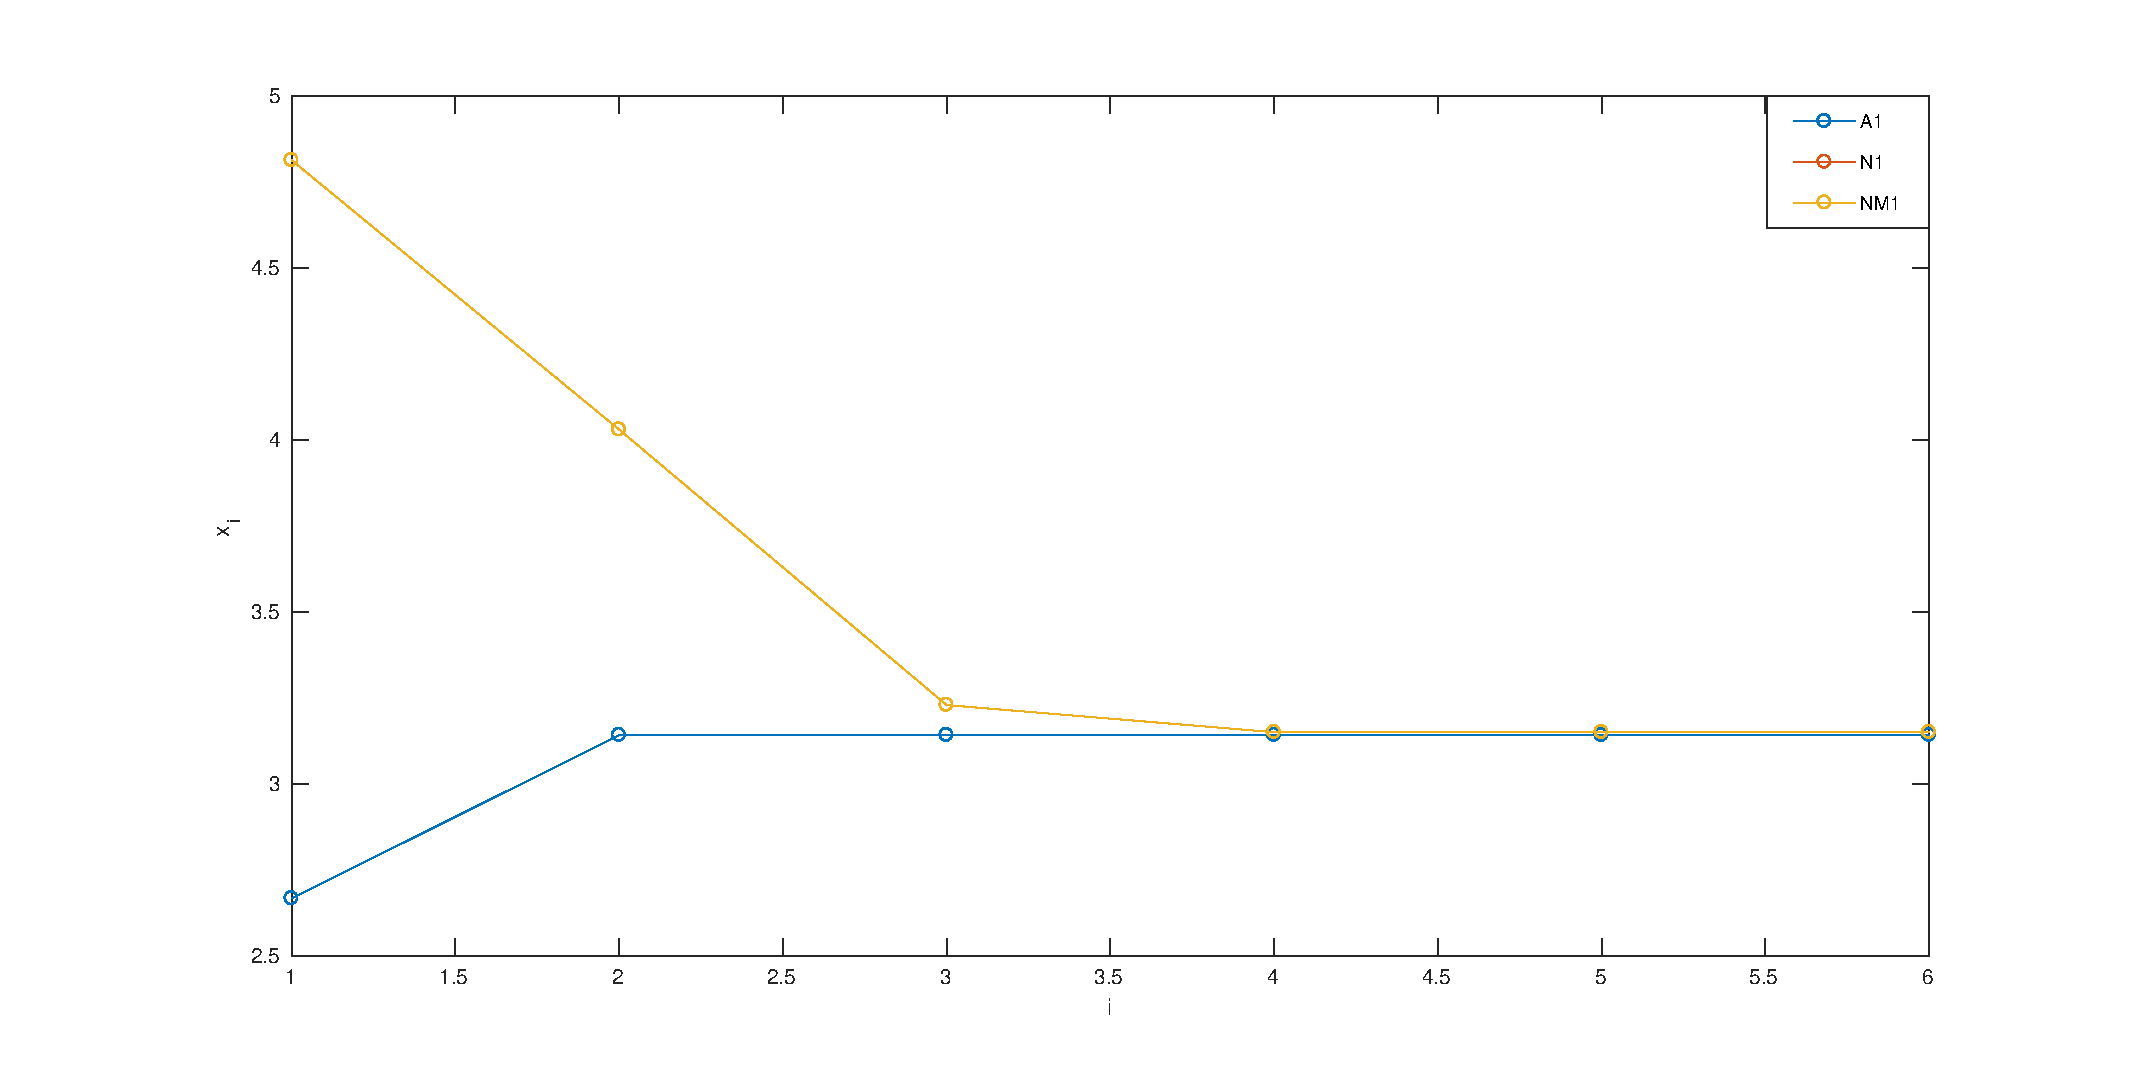
\includegraphics[left, width=210px]{plot/fes24a.eps}
\caption{Andamento del calcolo degli zeri della funzione $f_1(x)=(x-\pi)^{10}$ al variare della tolleranza}
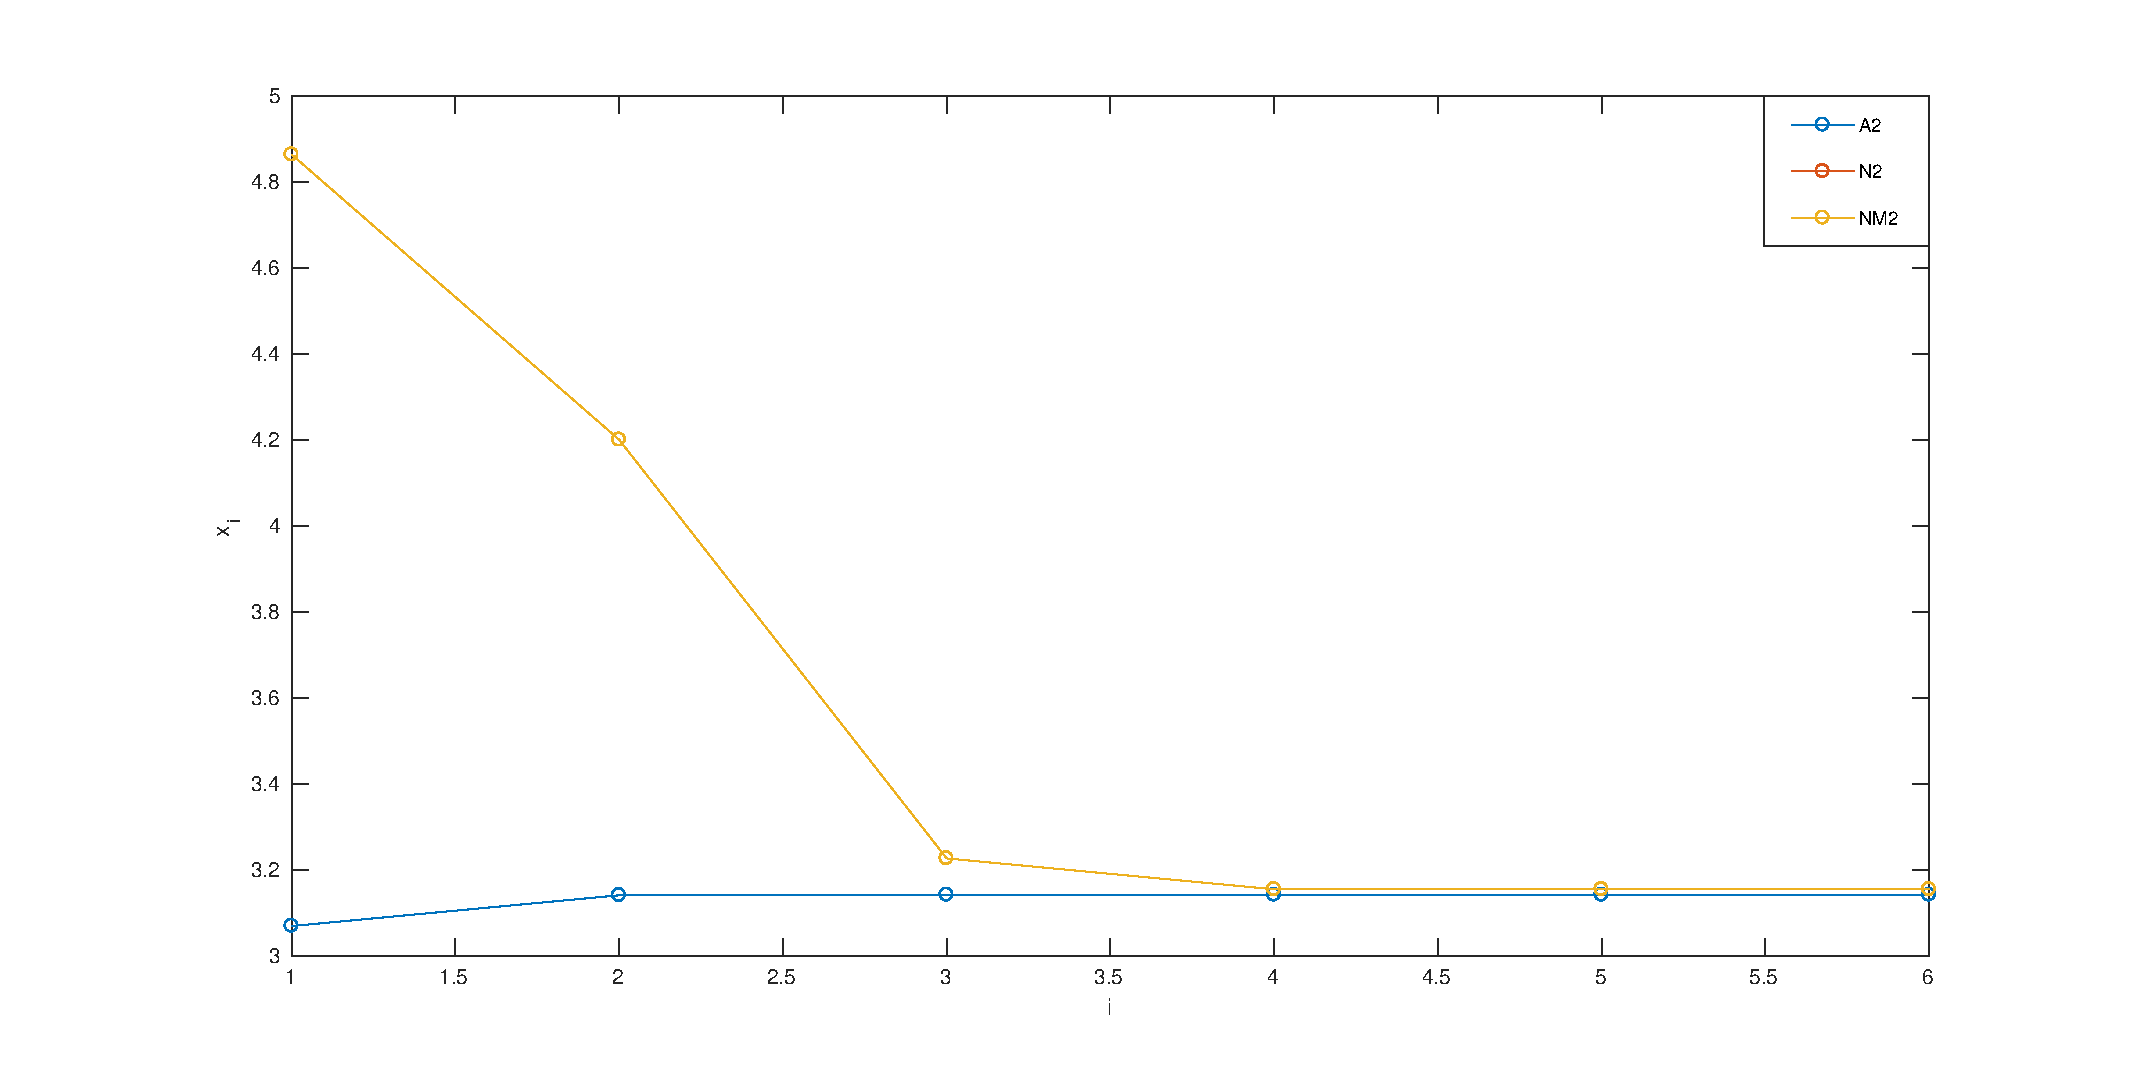
\includegraphics[left, width=210px]{plot/fes24b.eps}
\caption{Andamento del calcolo degli zeri della funzione $f_2(x) = (x-\pi)^{10} \cdot e^{2\cdot x}$ al variare della tolleranza}
\end{figure}
\end{flushleft}